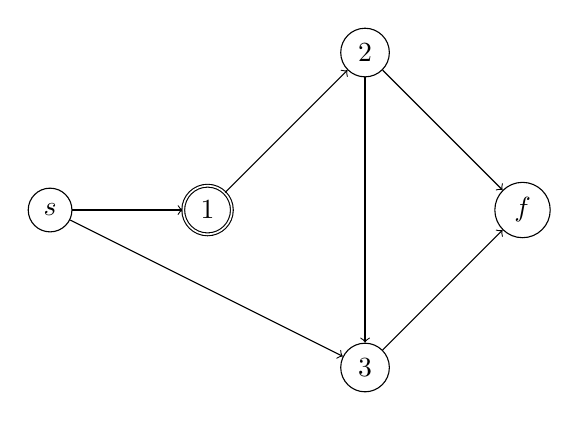
\begin{tikzpicture}[scale=2]
\node[draw,circle] (A) at (0,1) {$2$};
\node[draw,circle] (B) at (1,0) {$f$};
\node[draw,circle] (C) at (0,-1) {$3$};
\node[draw,circle,double] (D) at (-1,0) {$1$};
\node[draw,circle] (S) at (-2,0) {$s$};
\foreach \i/\j in {A/B,C/B,A/C,D/A,S/C,S/D} {
  \draw[->] (\i) -- (\j);
}
\end{tikzpicture}